\documentclass[10pt,a4paper]{article}

\usepackage[margin=1.5cm]{geometry}
\usepackage{graphicx}
\usepackage{multicol}
\usepackage{fancyhdr}
\usepackage{float}
\usepackage{listings}
\usepackage{xcolor}

\setlength{\columnsep}{0.6cm}

\pagestyle{fancy}
\fancyhf{}
\fancyfoot[R]{Page \thepage}
\renewcommand{\headrulewidth}{0pt}

\begin{document}

\begin{center}
    {\Large \textbf{Applied Robotics and Autonomous Systems}}

    \vspace{0.3cm}

    ACIT4820-1 26H

    \vspace{0.3cm}

    Nikolai Skaaheim-Grøna \\
    Lucas Van Der Horst \\
    Øyvind Amundsen Kjeang

    \vspace{0.3cm}

    Student numbers: 415337, 422009, oykje5980

    \vspace{0.2cm}

    ACIT Robotics and Control

    \vspace{0.1cm}

    OsloMet
\end{center}

\vspace{0.4cm}

\tableofcontents

\vspace{0.5cm}

\section{Introduction}

The aim of this assignment was to become familiar with ROS 2 and some of its basic tools. ROS 2 stands for Robot Operating System 2 and is a software framework that provides tools and communication methods for developing robotic systems. In this assignment, these tools were introduced by creating and visualizing a simple differential-drive robot consisting of a chassis, two drive wheels, and a caster wheel for support.

The robot was described using URDF (Unified Robot Description Format), a format used in ROS to describe the structure and physical parts of a robot. Links were used to represent the individual parts of the robot, while joints defined how these parts were connected.

The completed robot model was visualized in RViz, a visualization tool for displaying robot models and other data in ROS 2. TF (Transform) frames were also displayed to show the position and orientation of the different parts of the robot relative to each other.

A ROS 2 package was created to organize the files needed for the robot. This included the URDF file, launch file, and RViz configuration. The launch file was used to start the required components and open the model in RViz. In the final part of the assignment, a Python node was created to publish joint states, allowing the two drive wheels to rotate in the visualization.

Overall, the assignment provided a practical introduction to how a simple robot can be described, organized, and visualized in ROS 2, as well as how basic motion can be added to the model.


\section{Task 1: Create the URDF File}
The first part of the assignment started with creating a URDF file. This file describes what the robot looks like with links and joints. The URDF file format is a specific form of an XML file which is format in a text file. The convention for file extension is \texttt{.urdf}.

The assignment asked to model a differential-drive robot with a front caster wheel. So there are a few joints needed:

\begin{itemize}
    \item Base link
    \item Two cylinder wheels
    \item One caster wheel
    \item Base footprint
\end{itemize}

\subsection{Base link}
This is the body of the robot, all other parts will connect to this one. It's modelled visually by just a simple box. The code for this part looks like this:

\begin{lstlisting}[language=XML, basicstyle=\ttfamily\small, breaklines=true]
<link name="base_link">
	<visual>
	    <geometry>
		<box size="1 0.7 0.2" />
	    </geometry>
	</visual>
</link>
\end{lstlisting}

The dimensions of 1m long, by 70cm wide by 20cm tall were chosen pretty arbitrarily. 1 just seemed like the most basic number, and although maybe a little big for a robot, not unrealistic. The other proportions were then chosen to roughly match the proportions from the drawing in the assignment.

\begin{figure}[H]
    \centering
    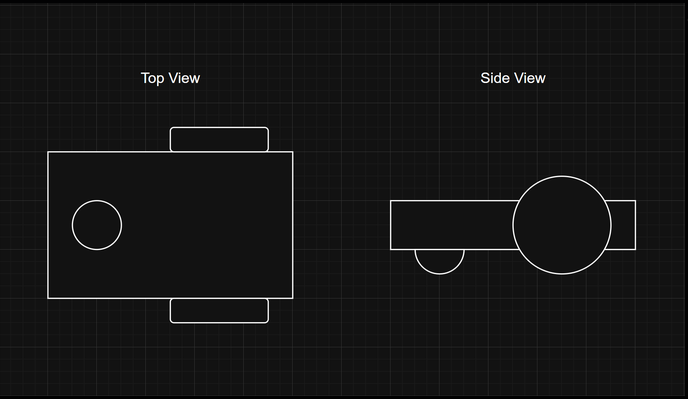
\includegraphics[width=0.7\linewidth]{Pictures/Robot_schematic.png}
    \caption{Robot schematic from the assignment.}
    \label{fig:robot-schematic}
\end{figure}

\subsection{Cylinder wheels}
Each drive wheel is a simple cylinder, visually. The wheel needs a \texttt{length} and \texttt{radius} 0.1 (10cm) for length and 0.2 (20cm) for radius were chosen, which seemed proportionate to the 20cm-tall base without looking oversized.

\begin{lstlisting}[language=XML, basicstyle=\ttfamily\small, breaklines=true]
<link name="left_wheel">
	<visual>
	    <geometry>
		<cylinder length="0.1" radius="0.2"/>
	    </geometry>
	</visual>
</link>
\end{lstlisting}

The joint is where the interesting part happens. A cylinder's default axis in URDF runs along its own local z-axis, but for a wheel to roll along the ground like a wheel rather than spin like a coin standing on its edge, its rotational axis needs to point sideways (along the robot's y-axis). So the \texttt{origin} in the joint applies an \texttt{rpy} rotation of \texttt{-1.57075} ($\approx -\pi/2$) around x, which tips the cylinder onto its side so it's oriented correctly relative to the base link.

The joint type is \texttt{continuous}, since a wheel needs to spin indefinitely in either direction, unlike a \texttt{revolute} joint which has limits. The \texttt{axis} is then given as \texttt{0 0 1}, this is in the joint's own rotated frame, so after the rpy rotation this axis now corresponds to the sideways direction of the wheel, letting it roll correctly.

The two wheels are placed symmetrically at $y = 0.40$ and $y = -0.40$, at $x = -0.3$ (toward the rear of the base), and their rpy signs are flipped between left and right so both wheels' outward face points away from the robot body.

\begin{lstlisting}[language=XML, basicstyle=\ttfamily\small, breaklines=true]
<joint name="base_link_to_left_wheel" type="continuous">
	<parent link="base_link"/>
	<child link="left_wheel"/>
	<origin xyz="-0.3 0.40 0" rpy="-1.57075 0 0"/>
	<axis xyz="0 0 1"/>
</joint>
\end{lstlisting}

\subsection{Caster wheel}
The caster wheel is modelled as a plain sphere rather than trying to represent an actual pivoting caster mechanism. This simplification was taken over from the assignment.

\begin{lstlisting}[language=XML, basicstyle=\ttfamily\small, breaklines=true]
<link name="caster_wheel">
	<visual>
	    <geometry>
		<sphere radius="0.15"/>
	    </geometry>
	</visual>
</link>
\end{lstlisting}

Since the swivel and roll of the caster aren't being modeled at all, the joint connecting it to \texttt{base\_link} is \texttt{fixed} --- it doesn't move relative to the base. It sits at the front of the robot, at $x = 0.3$ (opposite side from the drive wheels), and is dropped down slightly ($z = -0.05$) so that a 15cm-radius sphere reaches the ground.

\begin{lstlisting}[language=XML, basicstyle=\ttfamily\small, breaklines=true]
<joint name="base_link_to_caster_wheel" type="fixed">
	<parent link="base_link"/>
	<child link="caster_wheel"/>
	<origin xyz="0.3 0 -0.05" rpy="0 0 0"/>
</joint>
\end{lstlisting}

\subsection{Base footprint}
The assignment asked for this to be included but without much explanation. Looking it up, it seems to be a convention. If the base link were used as the origin, it would be like assuming that base\_link's origin already sits exactly on the ground with zero roll/pitch, and that it'll stay that way. So the base footprint is introduced to model the robot's position and angle relative to the ground.

To visualize this urdf file without having set up a package yet, just this one urdf file, the following command can be used, which reuses functionality from a tutorial package:

\begin{lstlisting}[language=bash, basicstyle=\ttfamily\small, breaklines=true]
ros2 launch urdf_tutorial display.launch.py model:=$(pwd)/my_robot.urdf
\end{lstlisting}

(For this, \texttt{ros-\$ROS\_DISTRO-urdf-tutorial} needs to be installed, which can be done via apt)

For reference, this is the whole urdf file:

\begin{lstlisting}[language=XML, basicstyle=\ttfamily\small, breaklines=true]
<?xml version="1.0"?>
<robot name="my_robot">
<link name="base_footprint"></link>
<link name="base_link">
<visual>
<geometry>
<box size="1 0.7 0.2" />
</geometry>
</visual>
</link>
<joint name="base_footprint_to_base_link" type="fixed">
<parent link="base_footprint"/>
<child link="base_link"/>
</joint>
<link name="left_wheel">
<visual>
<geometry>
<cylinder length="0.1" radius="0.2"/>
</geometry>
</visual>
</link>
<joint name="base_link_to_left_wheel" type="continuous">
<parent link="base_link"/>
<child link="left_wheel"/>
<origin xyz="-0.3 0.40 0" rpy="-1.57075 0 0"/>
<axis xyz="0 0 1"/>
</joint>
<link name="right_wheel">
<visual>
<geometry>
<cylinder length="0.1" radius="0.2"/>
</geometry>
</visual>
</link>
<joint name="base_link_to_right_wheel" type="continuous">
<parent link="base_link"/>
<child link="right_wheel"/>
<origin xyz="-0.3 -0.40 0" rpy="1.57075 0 0"/>
<axis xyz="0 0 1"/>
</joint>
<link name="caster_wheel">
<visual>
<geometry>
<sphere radius="0.15"/>
</geometry>
</visual>
</link>
<joint name="base_link_to_caster_wheel" type="fixed">
<parent link="base_link"/>
<child link="caster_wheel"/>
<origin xyz="0.3 0 -0.05" rpy="0 0 0"/>
</joint>
</robot>
\end{lstlisting}

\section{Task 2: Read the wiki}

This task could more accurately be described as ``Create your own package,'' since that is the primary activity involved. Reading the wiki was necessary to understand how to carry out this and the subsequent steps, and the slides from \texttt{C03\_packages\_colcon-1.pdf} proved to be the most useful resource.

The package template files and folder structure were created using the following command, taken from the slides:
\begin{lstlisting}[language=bash]
ros2 pkg create --build-type ament_python my_robot_description
\end{lstlisting}
This command must be run from inside the \texttt{src} folder created by colcon.

From the workspace root, the following commands were then run:
\begin{lstlisting}[language=bash]
colcon build
source install/setup.bash
\end{lstlisting}
Whenever changes are made within the package, the workspace must be rebuilt, and \texttt{install/setup.bash} must be sourced again in every open terminal.

As specified in the assignment, the subfolders \texttt{launch} and \texttt{urdf} were added to the package at \texttt{src/my\_robot\_description}. The URDF file created earlier was moved into the \texttt{urdf} folder, and a \texttt{display.launch.xml} file was created in the \texttt{launch} folder, to be completed in a later task. Before this, the new folders needed to be added to \texttt{data\_files} in \texttt{setup.py}, so that they would be included during the build. The resulting \texttt{data\_files} configuration was as follows:
\begin{lstlisting}[language=Python]
data_files=[
    ('share/ament_index/resource_index/packages', ['resource/' + package_name]),
    ('share/' + package_name, ['package.xml']),
    (os.path.join('share', package_name, 'urdf'), glob('urdf/*')),
    (os.path.join('share', package_name, 'launch'), glob('launch/*')),
]
\end{lstlisting}
Building was then tested by running \texttt{colcon build} again from the workspace root.

\section{Task 3: Visualization and TF Tree}

Once our URDF file was written, our next step was to visualize the robot and confirm that everything is structured correctly. We did this by creating a launch file named display.launch.xml that starts everything that we needed to visualize the robot in Rviz
\\
\\
Instead of writing a python script, we chose to write it in XML because Pierre recommended that the XML format is simpler. Python is more powerfull because it's a full programming language but it has more boilerplate code and we don't need it for this simpler project. Our launch file starts with three nodes:
\\
\\
\textbf{robot\_State\_Publisher}: reads our URDF file and published it to the ROS grapp so that tools like Rviz knows the robot structure and its connection with links 
\\
\\
\textbf{joint\_state\_publisher}: published the state of each joint. We used the GUI version so we could manually move the wheel joints with sliders.
\\
\\
\textbf{rviz2}: launched with a saved configuration file so the robot model and the transforms are displayed automatically so we dont need to do it manually every time we run it.
\\
\\
Once this was running, we could see the robot in Rviz: a rectangular chassis with two wheels on each side and a caster wheel. 

\subsection{Checking the TF tree}

while having the launch file running, we opened a second terminal and used:
\begin{lstlisting}[language=bash]
ros2 run tf2_tools view_frames
evince frames.pdf
\end{lstlisting}

This produced a PDF showing the full chain of frames:


\begin{figure}[H]
    \centering
    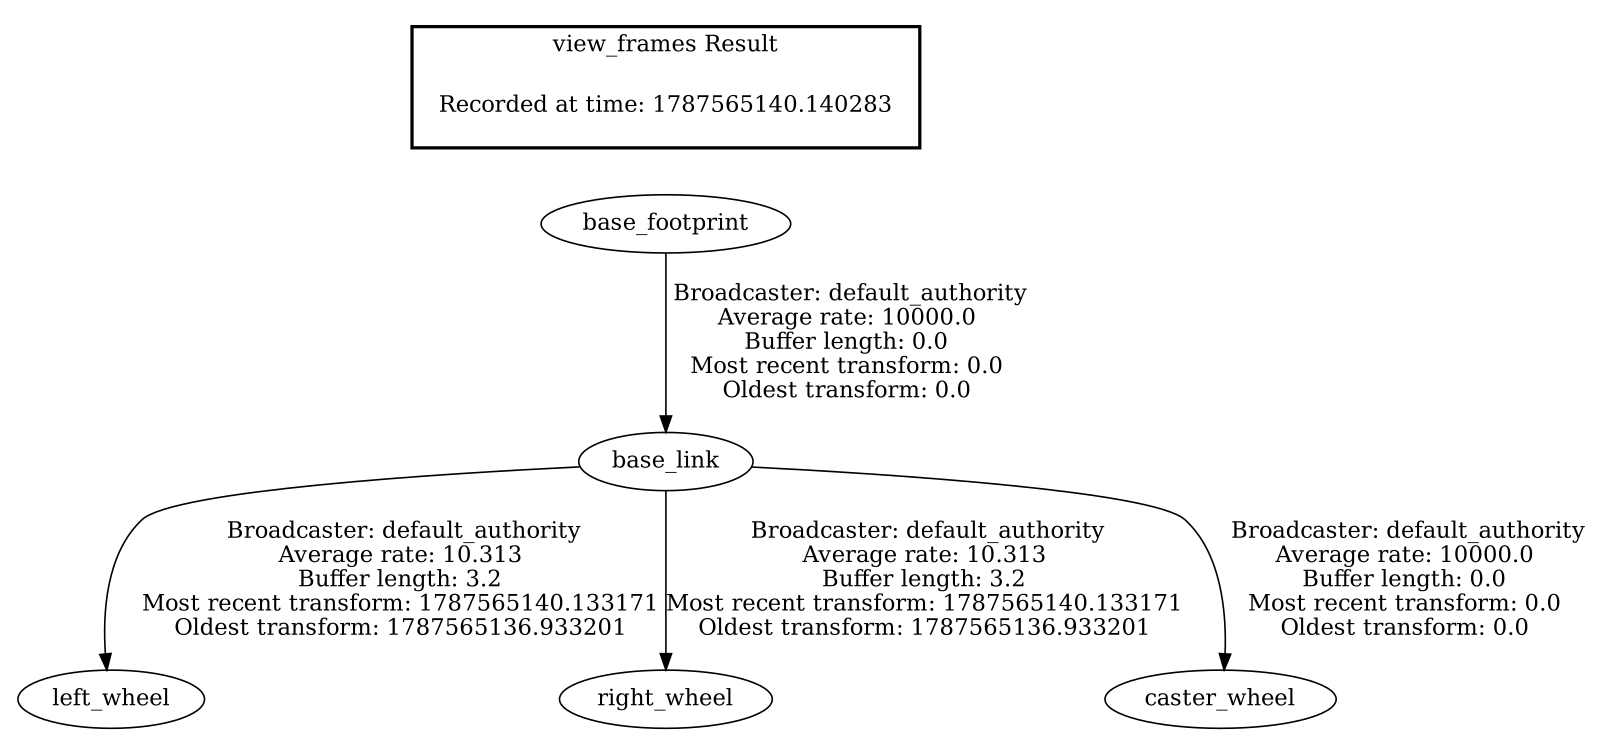
\includegraphics[width=0.7\textwidth]{Pictures/TFtree.png}
    \caption{TF tree of our robot model, generated with \texttt{tf2\_tools}.}
    \label{fig:tf_tree}
\end{figure}

The same frames were inspected spatially in RViz. We enabled TF axes and names to visually verify the frame position and orientation.

\begin{figure}[H]
    \centering
    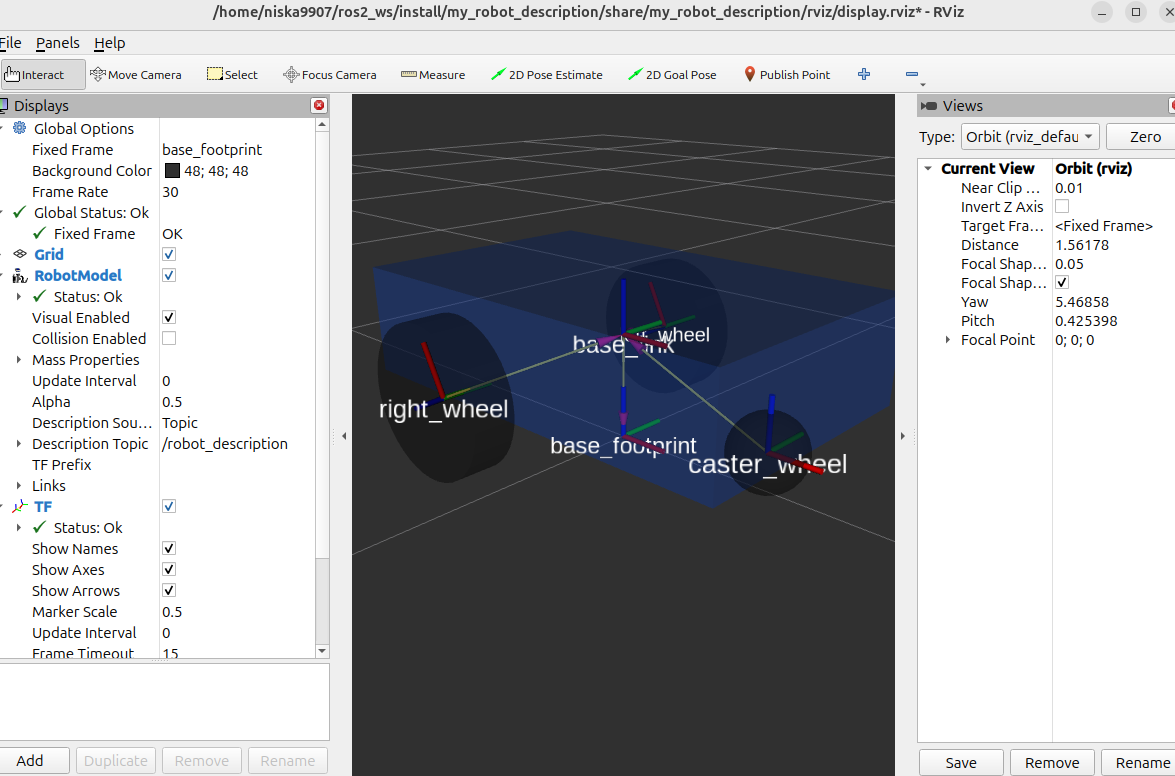
\includegraphics[width=0.7\textwidth]{Pictures/RobotPic.png}
    \caption{Robot model in RViz with TF axes and frame names displayed}
    \label{fig:tf_tree}
\end{figure}




\section{Task 4: Adding Wheel Motion}

For the final task, a Python node was created to make the two drive wheels rotate automatically. A Python node is a program that performs a specific task within a ROS 2 system and can send or receive data.

The \texttt{joint\_state\_publisher\_gui} used in the previous task was useful for manually testing the wheel joints, but it could not provide the automatic motion required in Task 4. Therefore, a separate Python node was created to continuously publish updated wheel positions to the \texttt{/joint\_states} topic using the \texttt{JointState} message type.

A timer was used to update the wheel positions every 0.1 seconds. Each time the function runs, the position is increased and the new position is published for both wheel joints.

\begin{figure}[H]
    \centering
    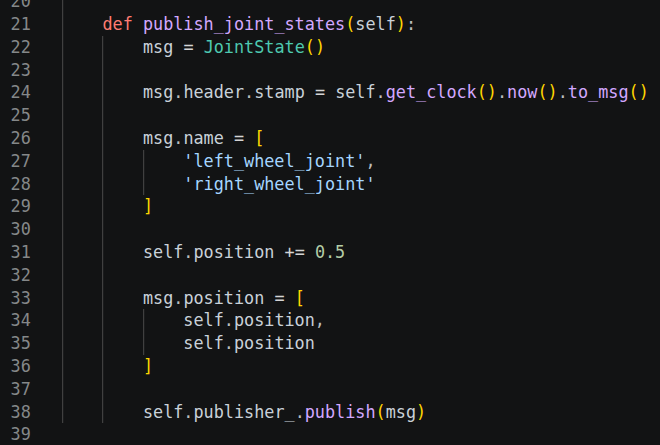
\includegraphics[width=0.5\linewidth]{Pictures/publish_joint_states.png}
    \caption{Python function publishing joint states for the left and right wheels.}
    \label{fig:placeholder}
\end{figure}


Both wheels are given the same position, so they rotate at the same speed. The caster wheel is not included because its joint is fixed.

The Python node was also added to the launch file instead of the \texttt{joint\_state\_publisher\_gui}. This makes the wheel publisher start automatically together with the rest of the robot.

\begin{figure}[H]
    \centering
    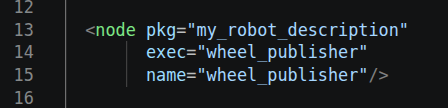
\includegraphics[width=0.5\linewidth]{Pictures/pkgrobotdescription.png}
    \caption{Launch file configuration for starting the wheel publisher node.}
    \label{fig:placeholder}
\end{figure}
    


To check that the node was working, the \texttt{/joint\_states} topic was viewed using:

\begin{lstlisting}[language=bash]
ros2 topic echo /joint_states
\end{lstlisting}

\begin{figure}[H]
    \centering

    \begin{minipage}{0.48\linewidth}
        \centering
        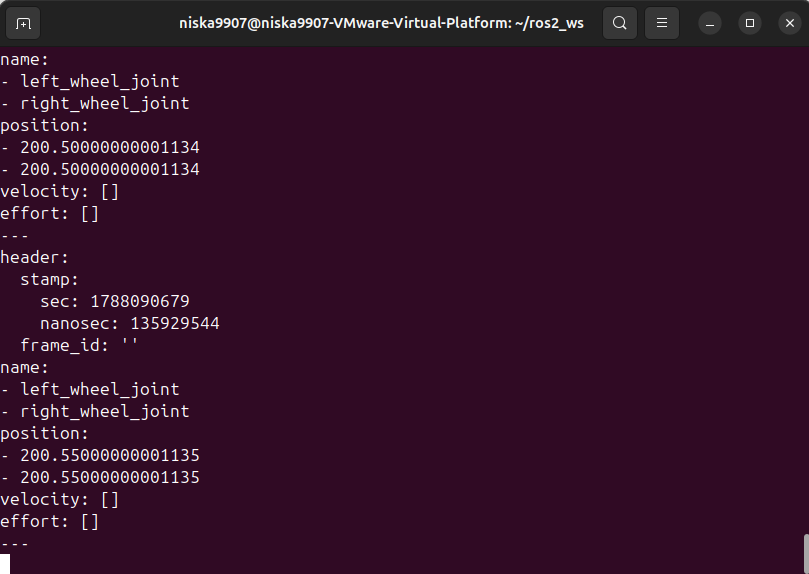
\includegraphics[width=\linewidth]{Pictures/Wheel_movement1.png}
    \end{minipage}
    \hfill
    \begin{minipage}{0.48\linewidth}
        \centering
        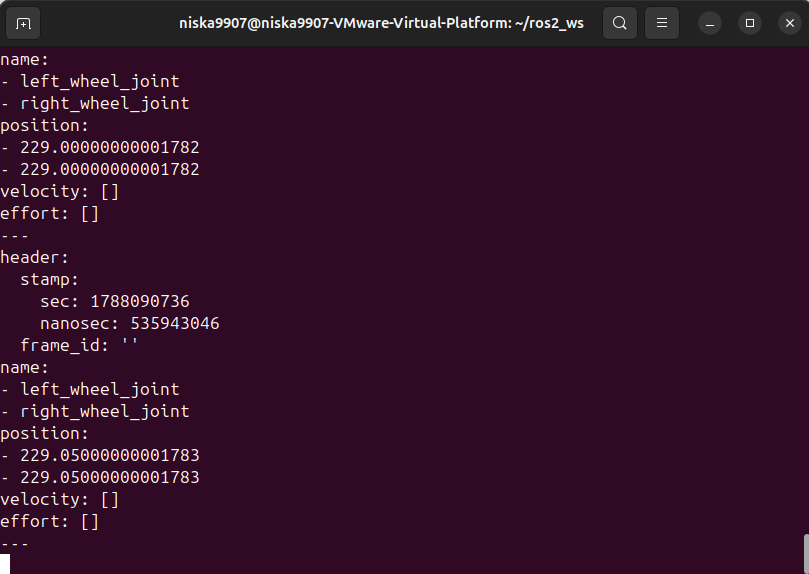
\includegraphics[width=\linewidth]{Pictures/Wheel_movement2.png}
    \end{minipage}

    \caption{Output from \texttt{/joint\_states} showing the position
values increasing for both wheel joints.}
    \label{fig:robot_visualization}
\end{figure}

The position values for both wheels increased continuously, showing that the node was publishing the wheel movement correctly. The wheels could then be visualized rotating in RViz.


\begin{figure}[H]
    \centering

    \begin{minipage}{0.48\linewidth}
        \centering
        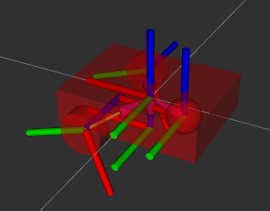
\includegraphics[width=\linewidth]{Pictures/Robotaxis.png}
    \end{minipage}
    \hfill
    \begin{minipage}{0.48\linewidth}
        \centering
        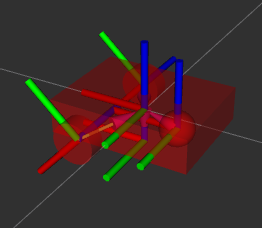
\includegraphics[width=\linewidth]{Pictures/Robotaxisafter.png}
    \end{minipage}

    \caption{Robot model in RViz with wheels spinning}
    \label{fig:robot_visualization}
\end{figure}

The communication between the nodes was inspected using \texttt{rqt\_graph}. the picture shows  the wheel publisher sending joint positions thorugh \texttt{joint\_states} to the \texttt{robot\_state\_publisher}, which publishes the resulting transforms to RViz through \texttt{/tf} and \texttt{/tf\_static}. the names \texttt{wheel\_publisher} and \texttt{wheel\_state\_publisher} are different because the group members worked separately and chose different names.Both of the nodes perform the same task.

\begin{figure}[H]
    \centering
    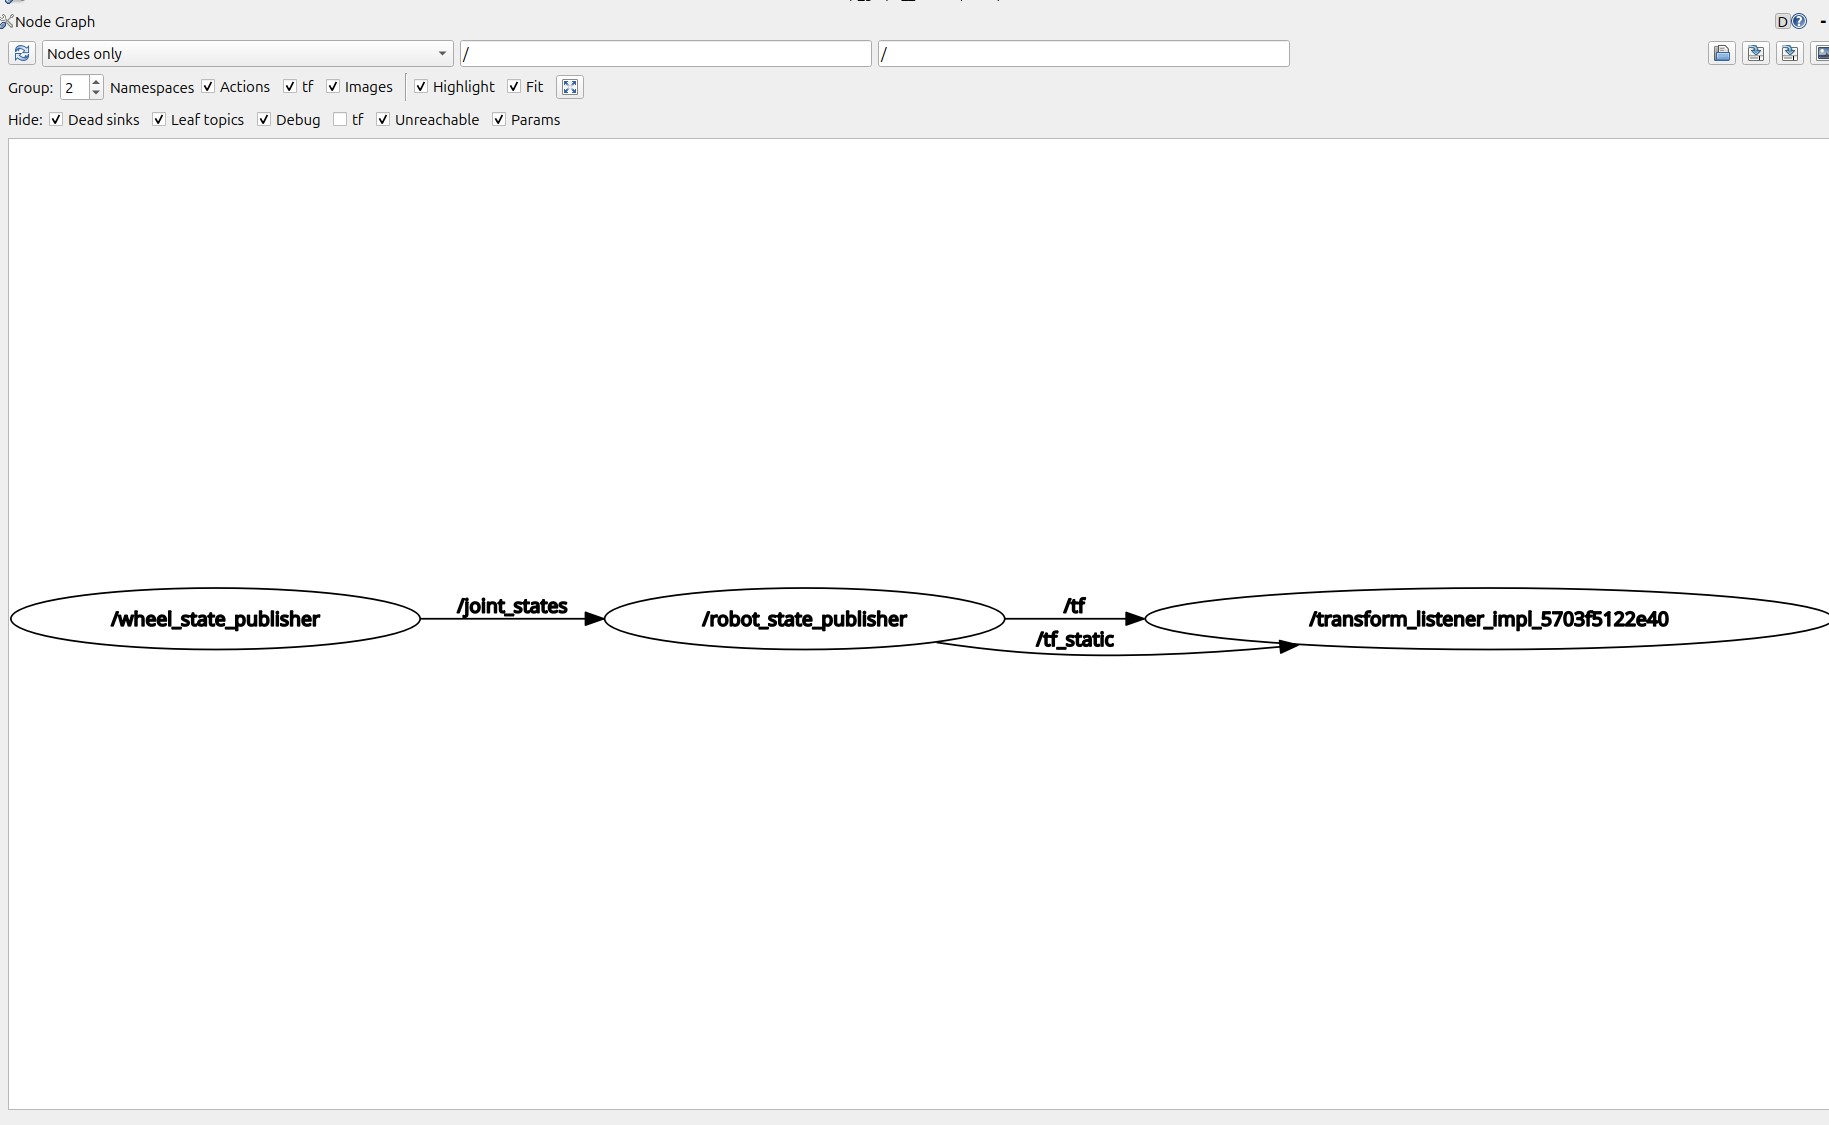
\includegraphics[width=0.5\linewidth]{Pictures/rqt_graph.png}
    \caption{ROS 2 node and topic communication visualized using
    \texttt{rqt\_graph}.}
    \label{fig:placeholder}
\end{figure}

During testing, the wheels did not initially appear to rotate in RViz. To determine whether the problem was caused by the Python node, the active nodes were checked using \texttt{ros2 node list}, and the \texttt{/joint\_states} topic was inspected using \texttt{ros2 topic echo /joint\_states}. The \texttt{wheel\_publisher} node was running and the position values increased continuously, confirming that the Python node was publishing correctly. This showed the importance of checking the individual parts of a ROS 2 system separately when troubleshooting, rather than assuming that a problem in the visualization is caused by the publisher.

\section{Problems Encountered and Solutions}

\textbf{Missing URDF and launch files after compiling.} After compilation, the URDF and launch files could not be found. This appeared to be the common issue of these files not being included in \texttt{data\_files} in \texttt{setup.py}. However, \texttt{setup.py} had already been modified to include them. After some investigation, it was discovered that the changes to \texttt{setup.py} had never actually been saved, which explained the behavior. This occurred because VS Code's autosave had failed silently, since \texttt{setup.py} (and several other files) only had write permissions for the root user. This, in turn, was because the \texttt{ament\_python} command had been run as root, meaning all files and directories it created also required root privileges to modify. Broadening the write permissions with \texttt{chmod} resolved the problem.

\textbf{GUIs not displaying from inside the Docker container.} Graphical user interfaces did not appear when launched from inside the Docker container. This was because the display output needed to be configured to be passed through to the host machine. This was resolved by adding the following configuration to \texttt{docker-compose.yaml}:
\begin{lstlisting}[language=bash]
environment:
  - DISPLAY=${DISPLAY}
  - QT_QPA_PLATFORM=xcb
  - QT_X11_NO_MITSHM=1
  - XDG_RUNTIME_DIR=/tmp/runtime-root
volumes:
  - /tmp/.X11-unix:/tmp/.X11-unix
devices:
  - /dev/dri:/dev/dri
group_add:
  - video
stdin_open: true
tty: true
\end{lstlisting}
and by running the following commands on the host machine:
\begin{lstlisting}[language=bash]
sudo apt install x11-xserver-utils
echo "xhost +local:root" >> ~/.bashrc
\end{lstlisting}

\vspace{0.4cm}

\begin{multicols}{2}

\end{multicols}

\end{document}